\documentclass[12pt]{article}
\usepackage{amsmath}
\usepackage{amssymb}
\usepackage{graphicx}
\usepackage{algorithm}
\usepackage{algpseudocode}% http://ctan.org/pkg/algorithmicx
\usepackage{xcolor}
\usepackage{geometry}
\usepackage{booktabs}
\usepackage{listings}
\usepackage{tocbibind} % To include index in the table of contents
%\usepackage{gvv}
\usepackage{gvv-book}
\geometry{a4paper, margin=1in}
\title{QR Algorithm based on SRA with Aggressive Deflation}
\author{EE24BTECH11059 - Y SIDDHANTH}
\definecolor{mygray}{rgb}{0.5,0.5,0.5}
\definecolor{mymauve}{rgb}{0.58,0,0.82}
\definecolor{myblue}{rgb}{0.13,0.13,0.6}
\lstset{
	language=C,
	backgroundcolor=\color{white},
	commentstyle=\color{mygray},
	keywordstyle=\color{myblue},
	numberstyle=\tiny\color{mygray},
	stringstyle=\color{mymauve},
	basicstyle=\ttfamily\small, % Change font size here
	breaklines=true,
	numbersep=8pt,
	showstringspaces=false,
	tabsize=4
}
\begin{document}
	
	\maketitle
	\tableofcontents % Generates the table of contents
	\clearpage
	
	\section{Introduction}
	This report documents the implementation of optimized matrix operations and making of the Schwarz Rutishauser Algorithm for QR decomposition in C, along side with the use of a self made complex arithmetic's library. The provided code is designed to perform operations such as matrix multiplication, scaling, addition, subtraction, transposition, and QR decomposition. The code is optimized using clever matrix multiplication algorithms and compiler flags such as \textbf{-O3} and \textbf{-ffast-math} for high-performance computing and efficient memory management by the use of globally declared to variables to avoid possible memory leaks. New variables such as \textbf{Convergence $\epsilon$} and \textbf{Deflation $\delta$} have been employed to make convergence faster while keeping the true eigen values unchanged and stable.
	\newpage
	\section{What is the QR Algorithm? \cite{5}}
	The QR algorithm computes a Schur decomposition of a matrix. It is certainly one of the most important algorithms in eigenvalue computations \cite{6}. However, it is applied to dense (or: full) matrices only.
	
	The QR algorithm consists of two separate stages. First, by means of a similarity transformation, the original matrix is transformed in a finite number of steps to Hessenberg form or -- in the Hermitian/symmetric case -- to real tridiagonal form. This first stage of the algorithm prepares its second stage, the actual QR iterations that are applied to the Hessenberg or tridiagonal matrix. The overall complexity (number of floating points) of the algorithm is \( O(n^3) \).
	\subsection{The basic QR algorithm}
	We notice first that
	\begin{equation}
		A_k = R_k Q_k = Q_k^* A_{k-1} Q_k,
	\end{equation}
	and hence $A_k$ and $A_{k-1}$ are unitarily similar. The matrix sequence $\{A_k\}$ converges (under certain assumptions) towards an upper hessenberg matrix .
	Let us assume that the eigenvalues are mutually different in magnitude and we can therefore number the eigenvalues such that $|\lambda_1| > |\lambda_2| > \cdots > |\lambda_n|$. 
	
	%From (\ref{eq:similarity}) we see that
	\begin{equation}
		A_k = Q_k^* A_{k-1} Q_k = Q_k^* Q_{k-1}^* A_{k-2} Q_{k-1} Q_k = \cdots = Q_k^* Q_{k-1}^* \cdots Q_1^* A_0 Q_1 \cdots Q_{k-1} Q_k.
	\end{equation}
	
	With the same assumption on the eigenvalues, $A_k$ tends to an upper hessenberg matrix.
	
	\begin{algorithm}[H]
		\caption{Basic QR algorithm}
		\label{alg:basic_qr}
		\begin{algorithmic}[1]
			\Require Let $A \in \mathbb{C}^{n \times n}$. This algorithm computes an upper hessenberg matrix $T$ and a unitary matrix $U$ such that $A = UTU^*$ is the Schur decomposition of $A$.
			\State Set $A_0 := A$ and $U_0 := I$.
			\For{$k = 1, 2, \ldots$}
			\State $A_{k-1} = Q_k R_k;$ \Comment{QR factorization}
			\State $A_k = R_k Q_k;$
			\State $U_k := U_{k-1} Q_k;$ \Comment{Update transformation matrix}
			\EndFor
			\State Set $T := A_{\infty}$ and $U := U_{\infty}.$
		\end{algorithmic}
	\end{algorithm}
	\subsection{The QR Algorithm with well chosen shifts}
	We notice first that
	\begin{equation}
		A_k = R_k Q_k = Q_k^* A_{k-1} Q_k,
	\end{equation}
	With a slight modification to our naive QR algorithm, we can reduce the computational cost significantly. This is by the use of shifts $\mu_k$.
	
	\begin{algorithm}[H]
		\caption{QR algorithm with Shifts}
		\begin{algorithmic}[1]
			\Require Let $A \in \mathbb{C}^{n \times n}$. This algorithm computes an upper triangular matrix $T$ and a unitary matrix $U$ such that $A = UTU^*$ is the Schur decomposition of $A$ using shifts.
			\State Set $A_0 := A$.
			\For{$k = 1, 2, \ldots$}
			\State $A_{k-1} = Q_k R_k - \mu_{k-1} I;$ \Comment{QR factorization}
			\State $A_k = R_k Q_k + \mu_{k-1} I;$
			\EndFor
			\State Set $T := A_{\infty}.$
		\end{algorithmic}
	\end{algorithm}
	\subsubsection{Rayleigh Quotient Iteration\cite{9}, \cite{10}}
	The Rayleigh quotient of a vector $\mathbf{x} \in \mathbb{R}^m$ is the scalar:
	\begin{equation}
		r(\mathbf{x}) = \frac{\mathbf{x}^T A \mathbf{x}}{\mathbf{x}^T \mathbf{x}} \label{eq:rayleigh_quotient}
	\end{equation}
	
	Notice that if $\mathbf{x}$ is an eigenvector, then $r(\mathbf{x}) = \lambda$ is the corresponding eigenvalue. One way to motivate this formula is to ask: given $\mathbf{x}$, what scalar $\alpha$ 
	"acts most like an eigenvalue" for $\mathbf{x}$ in the sense of minimizing $\| A\mathbf{x} - \alpha \mathbf{x} \|_2^2$? 
	
	This is an $n \times 1$ least squares problem of the form $A\mathbf{x} \approx \alpha \mathbf{x}$ 
	($A$ is the matrix, $\alpha$ is the unknown scalar, and $A\mathbf{x}$ is the right-hand side). By writing the normal equations (11.9) for this system, we obtain the answer: $\alpha = r(\mathbf{x})$. Thus, $r(\mathbf{x})$ is a natural eigenvalue estimate to consider if $\mathbf{x}$ is close to, but not necessarily equal to, an eigenvector.
	
	The idea is to use continually improving eigenvalue estimates to increase the rate of convergence of the QR iteration at every step. This algorithm is called Rayleigh quotient iteration.
		\begin{algorithm}[H]
		\caption{QR algorithm with Rayleigh Shifts}
		\begin{algorithmic}[1]
			\Require Let $A \in \mathbb{C}^{n \times n}$. This algorithm computes an upper triangular matrix $T$ and a unitary matrix $U$ such that $A = UTU^*$ is the Schur decomposition of $A$ using shifts.
			\State Set $A_0 := A$ and $x_0$ as some vector with $||x_0||= 1$
			\For{$k = 1, 2, \ldots$}
			\State $\mu_{k-1} = r(x_{k-1});$
			\State $A_{k-1} = Q_k R_k - \mu_{k-1} I;$ \Comment{QR factorization}
			\State $A_k = R_k Q_k + \mu_{k-1} I;$
			\State Find an $\omega$ for which $(A_k -\mu_{k-1} I)\omega = x_{k-1}$;
			\State $x_k = \omega / ||\omega||$;
			\EndFor
			\State Set $T := A_{\infty}.$ 
		\end{algorithmic}
	\end{algorithm}
	\subsection{How to find the complex eigen values of a real matrix?}
	We can clearly see that the Schur decomposition of a real matrix will always result in a real matrix. But if a real matrix were to have have complex eigen values, how would we find them? When computing the Schur, the principal diagonal is supposed to converged to the eigen values of the matrix and the matrix itself will converge into an upper triangular matrix. But if the eigen values of the matrix are complex, then the Schur of the matrix will converge to an \textbf{Upper Hessenberg Matrix}. Now the true complex eigen values will depend on the sub-diagonal above and below the principal diagonal containing the pseudo-eigen values.  
	\begin{algorithm}
		\caption{Eigenvalue Calculation}
		\label{eig}
		\begin{algorithmic}[1]
			\Require A matrix \( a \in \mathbb{R}^{n \times n} \)
			\Ensure Eigenvalues \( eig \)
			\State Initialize \( i = 0 \)
			\While{$i < n$}
			\If{(a[i+1][i] = 0 or a[i][i+1]  = 0)}
			\State $eig[i]  = a[i][i]$
			\State $i \rightarrow i + 1$
			\State continue
			\Else
			\State Extract the 2x2 submatrix \( M = \begin{pmatrix} a[i][i] & a[i][i+1] \\ a[i+1][i] & a[i+1][i+1] \end{pmatrix} \)
			\State Compute the trace and determinant of the submatrix:
			\State \( b \rightarrow a[i][i] + a[i+1][i+1] \) \quad (trace)
			\State \( c \rightarrow a[i][i] \cdot a[i+1][i+1] - a[i][i+1] \cdot a[i+1][i] \) \quad (determinant)
			\State \( \lambda_1, \lambda_2 = \frac{b \pm \sqrt{b^2 - 4c}}{2} \)
			\State Store the eigenvalues: \( eig[i] \rightarrow \lambda_1 \), \( eig[i+1] \rightarrow \lambda_2 \)
			\State \( i \rightarrow i + 2 \)
			\EndIf
			\EndWhile
		\end{algorithmic}
	\end{algorithm}
	\newpage
	\section{Schwarz Rutishauser Algorithm For QR Decomposition \cite{7}}
	\subsection{Gram Schmidt Algorithm and its drawbacks}
	This method is widely used for recursively finding an orthogonal matrix \( \mathbf{Q} \) of \( \mathbf{A} \), based on the orthogonal projection of each vector \( \mathbf{a}_k \in \mathbf{A} \), \( k=1\cdots n \) onto the span of vectors \( \mathbf{q}_i \in \mathbf{Q}^{(k)} \), \( i=1\cdots k \), that are already known. Each of the new orthogonal vectors \( \mathbf{q}_k \in \mathbf{Q} \) is computed as the sum of projections, subtracting it from the corresponding vector \( \mathbf{a}_k \in \mathbf{A} \). Finally, the upper triangular matrix \( \mathbf{R} \) can be easily obtained as the product of \( \mathbf{Q} \)'s-transpose and matrix \( \mathbf{A} \). 
	\begin{algorithm}
		\caption{Classical Gram-Schmidt (CGS)}
		\begin{algorithmic}[1]
			\Require Matrix \( A \in \mathbb{R}^{m \times n} \)
			\Ensure Orthonormal matrix \( Q \) and upper triangular matrix \( R \) such that \( A = QR \)
			\State Initialize \( Q = A \), \( R = 0_{n \times n} \)
			\For {\( k = 1 \) to \( n \)}
			\State Compute the norm: \( R[k,k] = \|Q[:,k]\| \)
			\State Normalize the column: \( Q[:,k] = Q[:,k] / R[k,k] \)
			\For {\( j = 1 \) to \( k-1 \)}
			\State Compute projection: \( R[k,j] = Q[:,k]^T \cdot Q[:,j] \)
			\State	Cumulative projection sum : \( S = S + R[k,j] \cdot Q[:,j] \)
			\EndFor
			\State $Q[:,k] = Q[:,k] - S$
			\EndFor \\
			\Return \( Q, R \)
		\end{algorithmic}
	\end{algorithm}\\
	The classical Gram-Schmidt orthogonalization is an enormously complex algorithm, caused by the computation of the orthogonal vector projection of each vector \( \mathbf{a}_k \in \mathbf{A} \) onto vectors \( \mathbf{q}_i \in \mathbf{Q}(k) \). In this case, the orthogonal projection operator complexity is about \( O(3m) \), and generally has a negative impact on the overall complexity of the Gram-Schmidt process. 
	
	\subsection{Schwarz Rutishauser's MGS} 
	The Schwarz-Rutishauser algorithm is a modification of the classical Gram-Schmidt orthogonalization process, proposed by H. R. Schwarz, H. Rutishauser and E. Stiefel, in their research paper “Numerik symmetrischer Matrizen” (Stuttgart, 1968) .  \cite{11}
	\begin{algorithm}
		\caption{Modified Gram-Schmidt (MGS)}
		\begin{algorithmic}[1]
			\Require Matrix \( A \in \mathbb{R}^{m \times n} \)
			\Ensure Orthonormal matrix \( Q \) and upper triangular matrix \( R \) such that \( A = QR \)
			\State Initialize \( Q = A \), \( R = 0_{n \times n} \)
			\For{\( k = 1 \) to \( n \)}
			\For{\( j = 1 \) to \( k-1 \)}
			\State Compute projection: \( R[k,j] = Q[:,k]^T \cdot Q[:,j] \)
			\State Subtract projection directly from \( Q[:,k] \): \( Q[:,k] = Q[:,k] - R[k,j] \cdot Q[:,j] \)
			\EndFor
			\State Compute the norm: \( R[k,k] = \|Q[:,k]\| \)
			\State Normalize the column: \( Q[:,k] = Q[:,k] / R[k,k] \)
			\EndFor \\
			\Return \( Q, R \)
		\end{algorithmic}
	\end{algorithm}
	\newpage
	\section{Convergence and Deflation}
	\subsection{Convergence}
		We know that the complex eigen values are dependent not only on the principal diagonal of the Schur of the input matrix, but also the sub-diagonal above and below it. We will conduct mainly 2 tests during every iteration of the QR algorithm. If either one of them are satisfied, then we will end the iterations and say that the Schur has been found.
		\subsubsection{Checking whether it has become Upper Hessenberg}
		This test is checks whether the current iteration has become an Upper Hessenberg Matrix. This may not be a very relevant test on it's own compared to the Convergence Epsilon Test, but paired with deflation, this test is very effective.
		\subsubsection{Convergence Epsilon}
		First, we store the norms of all the elements of the principal diagonal and the 2 sub-diagonals of the current iteration and the previous iteration. We will then create a divergence vector containing the difference of the norms of the current and previous elements.
		Now, we will define some $\epsilon$. When every element in the divergence vector is less than the $\epsilon$ we have defined, then we can say that the matrix has converged.\\ 
		The real question is, how do we find the $\epsilon$?\\
		For a $3\times 3$ and a $4 \times 4$ matrix with all single digit complex elements, we will experiment different epsilons, and find the number of iterations it takes to converge:
		\begin{table}[H]
			\centering
			\begin{minipage}{0.45\textwidth}
				\centering
				\begin{tabular}{|c|c|}
					\hline
					$\epsilon - 3$ & Iterations \\
					\hline
					1 & 4 \\
					1e-1 & 6 \\
					1e-2 & 6 \\
					1e-3 & 6 \\
					1e-4 & 6 \\
					1e-5 & 6 \\
					1e-6 & 6 \\
					1e-7 & 6 \\
					1e-8 & 6 \\
					\hline
				\end{tabular}
				\caption{Table for $\epsilon - 3$}
			\end{minipage}%
			\hspace{0.5cm}  % Space between the tables
			\begin{minipage}{0.45\textwidth}
				\centering
				\begin{tabular}{|c|c|}
					\hline
					$\epsilon - 4$ & Iterations \\
					\hline
					1 & 5 \\
					1e-1 & 15 \\
					1e-2 & 18 \\
					1e-3 & 25 \\
					1e-4 & 31 \\
					1e-5 & 37 \\
					1e-6 & 42 \\
					1e-7 & 42 \\
					1e-8 & 42 \\
					\hline
				\end{tabular}
				\caption{Table for $\epsilon - 4$}
			\end{minipage}
		\end{table}
		\textbf{High Accuracy Approach}: If number of iterations and computation time is insignficant, then keeping $\epsilon = 1e-15 \text{ or } 0$ is the best approach. It is guaranteed to give very accurate eigen values, but is very time consuming and resource draining. \\
		\textbf{High Performance Approach}: If number of iterations and computation time do matter, then keeping $\epsilon = 1e-4 $ or keeping the eigen values till 4 digits of accuracy is the best approach. This approach is good for applications satisfied with a fixed amount of accuracy in eigen values.

		Clearly for the $4\times 4$, the matrix converges at an $\epsilon = 1e-6$ where as for the $3\times 3$, it is $1e-1$. We can see that we have two approaches from here on, \textbf{High Accuracy} or \textbf{High Performance}.\\
		\subsubsection{Alternate Convergence Epsilon}
		In the original method we are comparing each element of the divergence vector to the convergence $\epsilon$. Rather we can compare the norm of the divergence vector to the convergence $\epsilon$.
		\subsection{Deflation}
		As the number of iterations increase in large matrices, the elements don't really converge to zero. Even after a horrendous amount of iterations, the elements which are supposed to become zero, become a very close value to zero.\\
		Example: Consider a $100 \times 100$ matrix, and now we will compute QR without the convergence tests. When the iteration number is 10000, we expect the matrix to converge into Upper Hessenberg, but instead of the zeroes we have incredibly small values like $1e-32, 1e-256, 1e-15$. \\
		To Solve this problem, we will consider a new variable, called the Deflation $\delta$. 
		\subsubsection{Deflation $\delta$}
		This effectively sets a "zero" or baseline for all the matrix operations. It is like a pseudo-zero. This doesn't effect the eigen values drastically, but the number of iterations are reduced considerably. The unnecessary calculations are avoided and the matrix is forced into Upper Hessenberg form faster. There are 3 apporaches for the value of $\delta$ in this case too, \textbf{High Accuracy}, \textbf{High Performance}, \textbf{High Precision}.\\\\
 		\textbf{High Accuracy}: High Accuracy can be obtained by just neglecting the use of $\delta$ or it can be achieved by keeping it at $$\delta = 1e-20$$. I have decided on this $\delta$ due to its consistent performance for larger matrices scaling upto $n = 800$.\\
 		\textbf{High Precision}: High Precision is the middle ground of high accuracy and high performance which can be obtained by defining $\delta$ as $$\delta = \frac{\epsilon}{max(a_{ij})}$$. The eigen values in this combination were stable and consistent for very large matrices too for $\epsilon = 1e-4$.\\
 		\textbf{High Performance}: High Performance can be obtained by defining $\delta$ as $$\delta = \frac{1}{max(a_{ij})}$$. The eigen values in this combination were not as stable and consistent as it was for the High Precision $\delta$ when it comes to large matrices in the scale of $n > 500$, but adequate accuracy was achieved for smaller matrices with a lesser amount of iterations.
 		
 		\subsubsection{Checking whether it has become Upper Hessenberg Pt. 2}
 		We can now clearly see the use for the Upper Hessenberg test now. By using the Deflation $\delta$, we are forcing the matrix into Upper Hessenberg, but that doesn't mean that the matrix has converged.
 	\newpage
 	\section{Matrix Multiplication Optimization \cite{12}}
 	Suppose we have matrix A, B, both with dimensions 1000 by 1000. Below are 6 implementations to compute A*B in C programming language.
 	\begin{lstlisting}
 		void mat_mult_ijk(double **A, double **B, double **C, int m, int p, int n);
 		void mat_mult_ikj(double **A, double **B, double **C, int m, int p, int n);
 		void mat_mult_jik(double **A, double **B, double **C, int m, int p, int n);
 		void mat_mult_jki(double **A, double **B, double **C, int m, int p, int n);
 		void mat_mult_kij(double **A, double **B, double **C, int m, int p, int n);
 		void mat_mult_kji(double **A, double **B, double **C, int m, int p, int n);
 	\end{lstlisting}
 	The implementation of \texttt{mat\_mult\_ijk} is as following. 
 	\begin{lstlisting}
 		void mat_mult_ijk(double **A, double **B, double **C, int m, int p, int n) {
 			int i, j, k;
 			for ( i = 0; i < m; i++ )
 			for ( j = 0; j < n; j++ )
 			for ( k = 0; k < p; k++ )
 			C[i][j] += A[i][k]*B[k][j];
 		}
 	\end{lstlisting}
 	
 	Other 5 implementations are the same, except the order of the i, j, k for loops. Note that there are 3! = 6 combinations of different orders of the for loops.\\The elapsed CPU running times for the 6 implementations are as following:
 	\begin{lstlisting}
 		Elapsed CPU time (mat_mult_ijk) = 12.1 seconds
 		Elapsed CPU time (mat_mult_ikj) = 7.82 seconds
 		Elapsed CPU time (mat_mult_jik) = 10.01 seconds
 		Elapsed CPU time (mat_mult_jki) = 17.73 seconds
 		Elapsed CPU time (mat_mult_kij) = 7.77 seconds
 		Elapsed CPU time (mat_mult_kji) = 16.91 seconds
 	\end{lstlisting}
 	Basically, we can see that the methods with the index j in the very inner loop achieve the best performance in terms of the running time, 7.82s and 7.77s respectively. The reason for this has to do with how the data is stored and accessed during the computation.
 	\newpage
 	\section{Performance Overview} 
 	\subsection{(Randomly Generated) Real and Symmetric Matrices}
 	\begin{figure}[h]
 		\centering
 		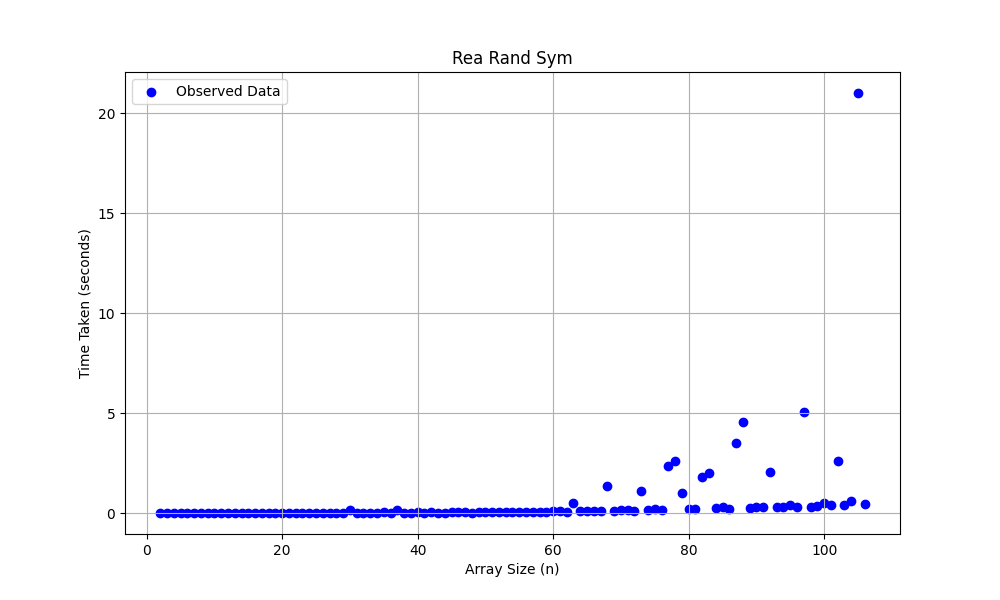
\includegraphics[width=0.85\textwidth]{figs/rrs.png}
 		\caption{Purely Real Randomly Generated Symmetric Matrix.}
 	\end{figure}
 	\subsection{(Randomly Generated) Real and Non-Symmetric Matrices}
 	\begin{figure}[h]
 		\centering
 		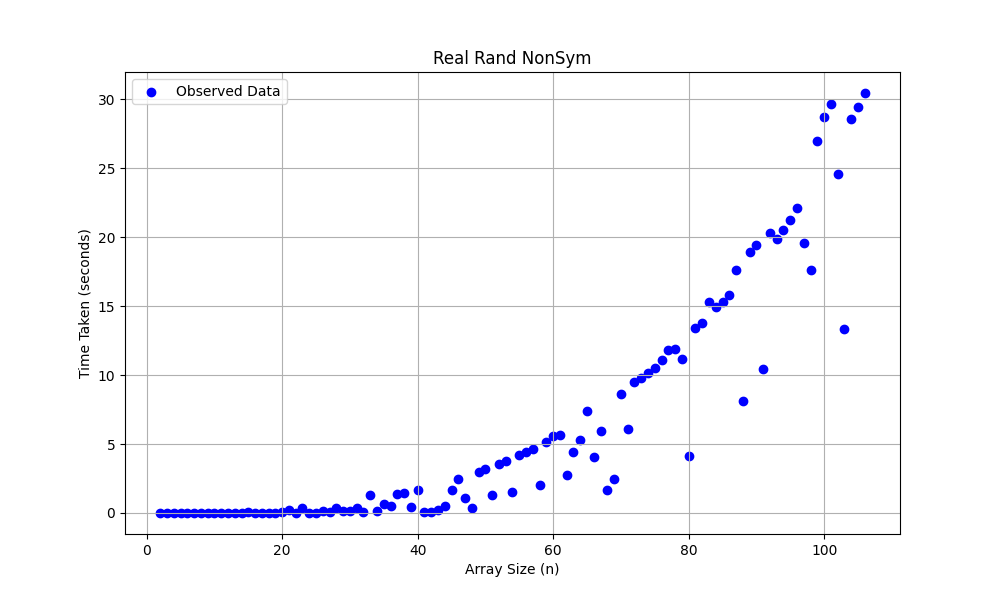
\includegraphics[width=0.85\textwidth]{figs/rrns.png}
 		\caption{Purely Real Randomly Generated Non-Symmetric Matrix.}
 	\end{figure}
 	\subsection{(Randomly Generated) Complex and Conjugate Symmetric Matrices}
 	\begin{figure}[h]
 		\centering
 		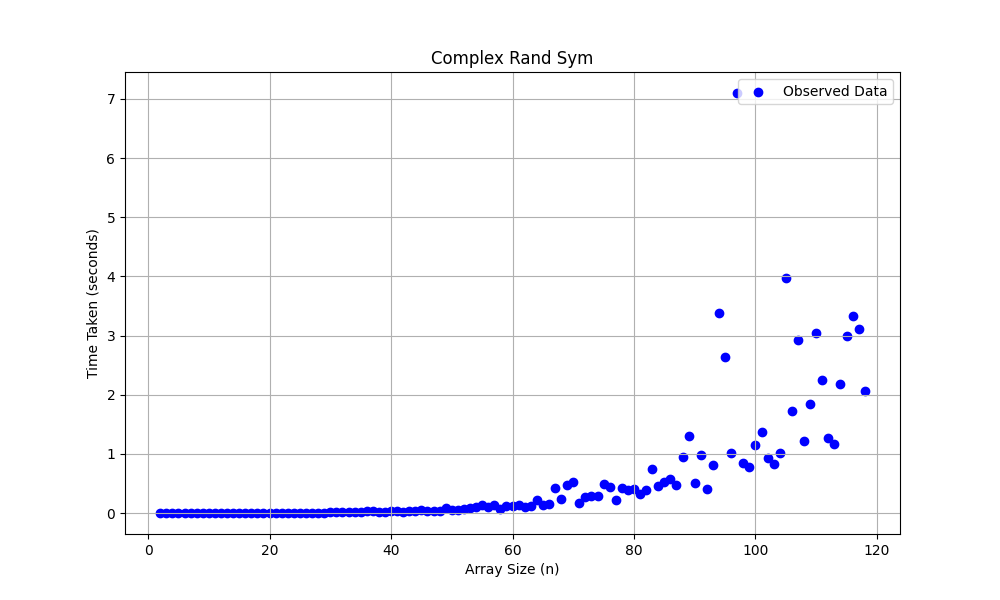
\includegraphics[width=0.85\textwidth]{figs/crs.png}
 		\caption{Complex Randomly Generated Conjugate Symmetric Matrix.}
 	\end{figure}
 	\subsection{(Randomly Generated) Complex and Non-Symmetric Matrices}
 	\begin{figure}[h]
 		\centering
 		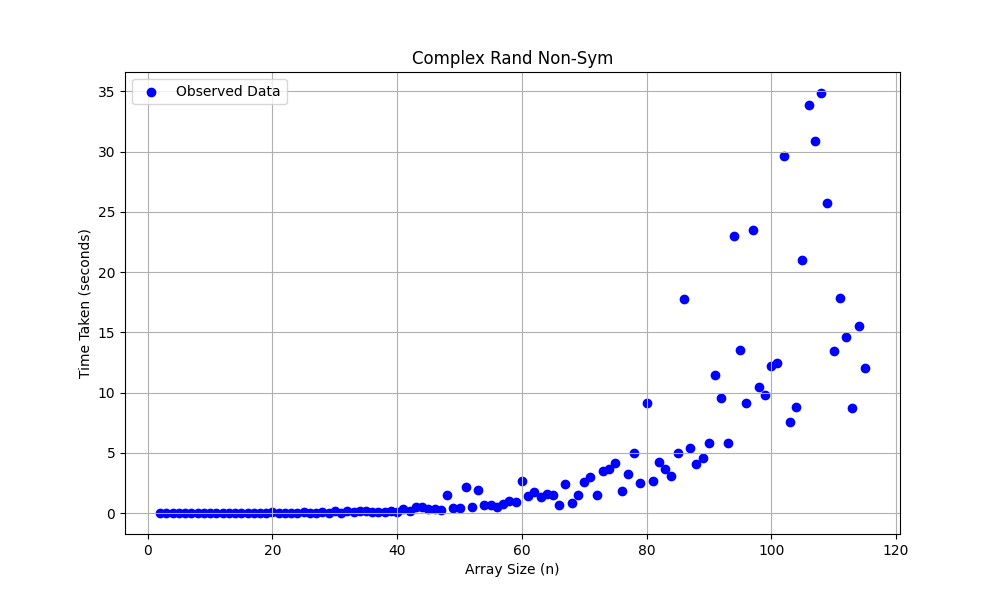
\includegraphics[width=0.85\textwidth]{figs/crns.png}
 		\caption{Complex Randomly Generated Non-Symmetric Matrix.}
 	\end{figure}
 	
 	\newpage
	\section{Code Overview}
	The implementation includes a set of functions defined in C to perform various matrix operations. The code is structured with a focus on complex number arithmetic.
	
	\subsection{Header Inclusions}
	The code starts by including essential libraries along side with the self-made complex arithmetic library:
	\begin{lstlisting}
		#include <stdio.h>
		#include <math.h>
		#include <stdlib.h>
		#include <time.h>
		#include <omp.h>
		#include <unistd.h>
		#include "evil.h"    -   Complex Arithmetics
		#include <string.h>
	\end{lstlisting}
	
	\subsection{Global Constants and Variables}
	A set of global constants and variables are defined to prevent memory leaks from happening and to reduce the number of inputs to functions.
	\begin{lstlisting}
		#define n 60
		#define epsilon 1e-4
		#define delta 1e-15
		
		double t[n][n][2] = {0};
		double t1[n][n][2] = {0};
		double t2[n][n][2] = {0};
		double qi[n][2];
		double qj[n][2];
		double tt[2];
		double eig[n][2];
		double null[2] = {0,0};
		double b[2] = {0}, c[2] = {0};
		double roots[2][2] = {0};
		double currpd[n] = {0};
		double currapd[n-1] = {0};
		double currbpd[n-1] = {0};
		double prevpd[n] = {0};
		double prevapd[n-1] = {0};
		double prevbpd[n-1] = {0};
		double diffpd[n] = {0};
		double diffapd[n-1] = {0};
		double diffbpd[n-1] = {0};
		
		//EVIL.H VARIABLES
		double temp1[2];     
		double temp2[2];
		double stemp[2];
	\end{lstlisting}
	\subsection{Evil Functions (Complex Arithmetic)}
	The complex arithmetic functions implemented in the code include:
	
	\subsubsection{Evil Addition}
	This function adds two complex numbers.
	\begin{lstlisting}
		double *eviladd(double z1[2],double z2[2]){
			temp1[0] = z1[0]+z2[0];
			temp1[1] = z1[1]+z2[1];
			return temp1;
		}
	\end{lstlisting}
	\subsubsection{Evil Subtraction}
	This function subtracts two complex numbers.
	\begin{lstlisting}
		double *evilsub(double z1[2],double z2[2]){
			temp1[0] = z1[0]-z2[0];
			temp1[1] = z1[1]-z2[1];
			return temp1;
		}
	\end{lstlisting}
	\subsubsection{Evil Multiplication}
	This function multiplies two complex numbers.
	\begin{lstlisting}
		double *evilmult(double z1[2],double z2[2]){
			stemp[0] = z1[0]*z2[0] - (z1[1]*z2[1]);
			stemp[1] = z1[0]*z2[1] + (z1[1]*z2[0]);
			return stemp;
		}
	\end{lstlisting}
	\subsubsection{Evil Division}
	This function divides two complex numbers.
	\begin{lstlisting}
		double *evildivi(double z1[2], double z2[2]){
			if(z1[0]==1 && z2[0]==0){
				temp1[0] = z2[0];
				temp1[1] = z2[1];
				return temp1;
			}
			double z2n = evilnormsq(z2);
			temp1[0] = (z1[0]*z2[0] + (z1[1]*z2[1]))/z2n;
			temp1[1] = (z1[1]*z2[0] - (z1[0]*z2[1]))/z2n;
			return temp1;
		}
	\end{lstlisting}
		\subsubsection{Evil Squared Magnitude}
	This function computes the squared magnitude of a complex number.
	\begin{lstlisting}
		double evilnormsq(double z1[2]){
			return z1[0]*z1[0] +(z1[1]*z1[1]);
		}
	\end{lstlisting}
	\subsubsection{Evil Conjugate}
	This function computes the conjugate of a complex number.
	\begin{lstlisting}
		double *evilcon(double z1[2]){
			temp2[0] = z1[0];
			temp2[1] = -z1[1]; 
			return temp2;
		}
	\end{lstlisting}
	\subsubsection{Evil Scaled Complex}
	This function computes the scaled version of a complex number.
	\begin{lstlisting}
		double *evilscale(double a[2],double k){
			temp1[0] = a[0]*k;
			temp1[1] = a[1]*k;
			return temp1;
		} 
	\end{lstlisting}
	\subsubsection{Evil Equator}
	This function copies one complex number to another.
	\begin{lstlisting}
		void evilequal(double z1[2], double z2[2]){
			z1[0] = z2[0];
			z1[1] = z2[1];
		}
	\end{lstlisting}
	\subsubsection{Equality Checker}
	This function checks whether the inputted complex numbers are equal.
	\begin{lstlisting}
		int isevilequal(double z1[2], double z2[2]){
			if(z1[0] == z2[0] && z1[1] == z2[1]) return 1;
			else return 0;
		}
	\end{lstlisting}
	\subsubsection{Evil Square Root calculator}
	This function computes the square root of a complex number.
	\begin{lstlisting}
		double *evilsqrt(double z1[2]) {
			double magnitude = sqrt(sqrt(evilnormsq(z1)));
			double angle = atan2(z1[1], z1[0]) / 2; 
			stemp[0] = magnitude * cos(angle);
			stemp[1] = magnitude * sin(angle);
			return stemp;
		}
	\end{lstlisting}
	\subsection{Matrix And Vector Functions}
	The core matrix functions implemented in the code include:
	
	\subsubsection{Nuller Function}
	This function resets the elements of an array to zero.
	\begin{lstlisting}
		void nuller(int N, double a[N]) {
			for (int i = 0; i < N; i++) {
				a[i] = 0;
			}
		}
	\end{lstlisting}
	
	\subsubsection{Matrix Multiplication}
	Performs matrix multiplication and accumulates results in a temporary array.
		\begin{lstlisting}
			void matmult(double a[n][n][2], double b[n][n][2], double p[n][n][2]) {
				for (int i = 0; i < n; i++) {
					for (int j = 0; j < n; j++) {
						nuller(2, t[i][j]);
					}
				}
				int i, j, k;
				double temp[2];
				for (i = 0; i < n; i++) {
					for (k = 0; k < n; k++) {
						for (j = 0; j < n; j++) {
							evilequal(t[i][j], eviladd(t[i][j], evilmult(a[i][k], b[k][j])));
						}
					}
				}
				for (int i = 0; i < n; i++) {
					for (int j = 0; j < n; j++) {
						evilequal(p[i][j], t[i][j]);
					}
				}
			}
		\end{lstlisting}
	
	\subsubsection{Matrix Scaling}
	Scales the elements of a matrix by a constant factor.
	\begin{lstlisting}
		void matscale(double a[n][n][2], double k) {
			for (int i = 0; i < n; i++) {
				for (int j = 0; j < n; j++) {
					evilequal(a[i][j], evilscale(a[i][j], k));
				}
			}
		}
	\end{lstlisting}
	
	\subsubsection{Matrix Addition}
	
	Computes the sum of two matrices.
	\begin{lstlisting}
		void matadd(double a[n][n][2], double b[n][n][2], double c[n][n][2]){
			for(int i=0;i<n;i++){
				for(int j=0;j<n;j++){
					evilequal(t1[i][j],eviladd(a[i][j], b[i][j]));
					evilequal(c[i][j], t1[i][j]);
				}
		}
	\end{lstlisting}
	\subsubsection{Matrix Subtraction}
	Computes the difference of two matrices.
	\begin{lstlisting}
		void matadd(double a[n][n][2], double b[n][n][2], double c[n][n][2]){
			for(int i=0;i<n;i++){
				for(int j=0;j<n;j++){
					evilequal(t1[i][j],evilsub(a[i][j], b[i][j]));
					evilequal(c[i][j], t1[i][j]);
				}
			}
		\end{lstlisting}
	\subsubsection{Matrix EYE}
	Creates a scaled identity matrix.
	\begin{lstlisting}
		void eye(double a[n][n][2], double k[2]){
			for(int i=0; i<n;i++){
				for(int j=0;j<n;j++){
					a[i][j][0] = (i==j)?k[0]:0;
					a[i][j][1] = (i==j)?k[1]:0;
				}
			}
		}
		\end{lstlisting}
	\subsubsection{Vector Insertion}
	Inserts a Vector into the i-th column of Matrix
	\begin{lstlisting}
		void ithcoltoarr(int i, double qi[n][2], double q[n][n][2]){
			for(int j=0; j<n;j++){
				evilequal(q[j][i],qi[j]);
			}
		}
		\end{lstlisting}
		\subsubsection{Vector Extraction}
	Extracts a Vector from the i-th column of Matrix
	\begin{lstlisting}
		void ithcoltoarr(int i, double qi[n][2], double q[n][n][2]){
			for(int j=0; j<n;j++){
				evilequal(qi[j], q[j][i]);
			}
		}
	\end{lstlisting}
	\subsubsection{Complex Inner Product}
	Computes the inner product of two vectors with complex elements.
	\begin{lstlisting}
		double *inner(double a[n][2], double b[n][2]){
			tt[0] = 0; tt[1] = 0;
			for(int i=0;i<n;i++){
				evilequal(tt,eviladd(tt,evilmult(evilcon(a[i]),b[i])));
			}
			return tt;
		}
	\end{lstlisting}
	\subsubsection{Complex Norm}
	Computes the norm of a vector with complex elements.
	\begin{lstlisting}
		double norm(double a[n][2]){
			double sum=0;
			for(int i=0;i<n;i++){
				sum += (a[i][1]*a[i][1]) + a[i][0]*a[i][0];
			}
			return sqrt(sum);
		}
	\end{lstlisting}
	\subsubsection{Matrix Printing Function}
	Prints out all the elements of a matrix in the exponential form..
	\begin{lstlisting}
		void printmat(double A[n][n][2]){
			for(int i=0;i<n;i++){
				for(int j=0; j<n;j++){
					printf("(%e , %e) ",A[i][j][0],A[i][j][1]);
				}
				printf("||\n");
				printf("\n");
			}
		}
	\end{lstlisting}
	\subsubsection{Vector Printing Function}
	Prints out all the elements of a vector in the exponential form..
	\begin{lstlisting}
		void printvec(double A[n][2]){
			for(int j=0; j<n;j++){
				printf("(%e , %e)\n",A[j][0],A[j][1]);
			}
		}
	\end{lstlisting}
	\subsection{Convergence Functions}
	The convergence checking matrix functions implemented in the code include:
	
	\subsubsection{Principal Diagonal and Subdiagonal Extractor}
	This function extracts the norm of the Principal Diagonal elements and the Subdiagonals above and below the PD. It stores them in their respective global variables.
	\begin{lstlisting}
		void extractpd(double A[n][n][2]){
			for(int i=0;i<n;i++){
				if(i<n-1){
					currbpd[i] = sqrt(evilnormsq(A[i+1][i]));
					currapd[i] = sqrt(evilnormsq(A[i][i+1]));
					currpd[i] = sqrt(evilnormsq(A[i][i+1]));
				} 
				else currpd[i] = sqrt(evilnormsq(A[i][i+1]));
			}
		}
	\end{lstlisting}
		\subsubsection{Principal Diagonal and Subdiagonal Updater}
	This function updates the norm of the Principal Diagonal elements and the Subdiagonals above and below the PD by  storing the current values in the previous values global variable.
	\begin{lstlisting}
		void updatepd(void){
			for(int i=0;i<n;i++){
				if(i<n-1){
					prevbpd[i] = currbpd[i];
					prevapd[i] = currapd[i];
					prevpd[i] = currpd[i];
				} 
				else prevpd[i] = currpd[i];
			}
		}
	\end{lstlisting}
		\subsubsection{Principal Diagonal and Subdiagonal Divergence Vector Calculator}
This function calculates the difference between the vectors storing the current diagonal norm and the previous diagonal norm.  The prev global variables are initiated to zero for the first iteration.
\begin{lstlisting}
	void pdsub(void){
		for(int i=0;i<n;i++){
			if(i<n-1){
				diffbpd[i] = currbpd[i] - prevbpd[i];
				diffapd[i] = currapd[i] - prevapd[i];
				diffpd[i] = currpd[i] - prevpd[i];
			}
			else diffpd[i] = currpd[i] - prevpd[i];
		}
	}
\end{lstlisting}
	\subsubsection{Hessenberg Checking Function}
	This function checks whether the input matrix is in the form of an upper-hessenberg matrix.
	\begin{lstlisting}
		int isHessenberg(double A[n][n][2]) {
			for (int i = 2; i < n; i++) {
				for (int j = 0; j < i - 1; j++) {
					if (A[i][j][0] != 0 || A[i][j][1] != 0) {
						return 0;
					}
				}
			}
			return 1;
		}
	\end{lstlisting}
	\subsubsection{Convergence Checking Function}
	This is the star of the show. It extracts the diagonals, calculates the divergence vectors and updates the global variables. After that, it checks whether all the elements in the divergence vectors are smaller that the \textbf{Convergence $\epsilon$}.
	\begin{lstlisting}
		int isConverged(double A[n][n][2]){
			extractpd(A);
			pdsub();
			updatepd();
			for(int i=0;i<n;i++){
				if(i<n-1){
					if(fabs(diffpd[i]) > epsilon) || fabs(diffapd[i]) > epsilon || fabs(diffbpd[i]) > epsilon){
							return 0;
						}
					}
				}
				return 1;
			}
	\end{lstlisting}
	\subsection{Deflation Functions}
	The matrix deflating functions implemented in the code include:
	
	\subsubsection{Matrix Deflate}
	This function checks changes all the elements of the input matrix which are less than the \textbf{Deflation $\delta$}
	\begin{lstlisting}
		void deflate(double A[n][n][2]){
			for(int i=0;i<n;i++){
				for(int j=0;j<n;j++){
					if(fabs(sqrt(evilnormsq(A[i][j]))) < delta) evilequal(A[i][j], null);
					else continue;
				}
			}		
		}
	\end{lstlisting}
	\subsection{Eigen Value Relevant Functions}
	\subsubsection{Naive Schur Calculation}
	This functions calculates the schur of a matrix without any shifts.
	\begin{lstlisting}
		int schur(double A[n][n][2]){
			double Q[n][n][2]={0}, R[n][n][2]={0}; int i= 0;
			while(i<10000000){
				qr(A,Q,R);
				matmult(R,Q,A);
				deflate(A);
				if(isConverged(A) || isHessenberg(A)){
					return i+1;
				}
				else i++;
			}
			return i;
		}
	\end{lstlisting}
	\subsubsection{Schur Calculation with Shifts}
	This functions calculates the schur of a matrix with a shift.
	\begin{lstlisting}
		int schurshift(double A[n][n][2]){
			double Q[n][n][2]={0}, R[n][n][2]={0}, U[n][n][2]; int i=0;
			while(i<10000){
				eye(U,A[n-1][n-1]);
				matsub(A,U,A);
				qr(A,Q,R);
				matmult(R,Q,A);
				matadd(A,U,A);
				deflate(A);
				if(isConverged(A) || isHessenberg(A)){
					return i+1;
				}
				else i++;
			}
			return i;
		}
	\end{lstlisting}
	\subsubsection{Eigen Value Calculator From Schur}
	It calculates the eigen values of computed Schur using the Algorithm \ref{eig}.
	\begin{lstlisting}
		void eigen(double a[n][n][2]){
			int i=0;
			while(i<n){
				if(isevilnull(a[i+1][i]) || isevilnull(a[i][i+1])){
					evilequal(eig[i], a[i][i]);i++;
					continue;
				}
				else{
					evilequal(tt, evilmult(a[i][i], a[i+1][i+1]));
					evilequal(c, evilsub(tt,evilmult(a[i+1][i], a[i][i+1]))); tt[0] = 0; tt[1] = 0;
					//printf("%lf\n",c[0]);
					evilequal(b, eviladd(a[i][i], a[i+1][i+1]));
					root(); //-> Finds the roots using the complex quadratic formula, and stores it in the roots[2]
					evilequal(eig[i], roots[0]);evilequal(eig[i+1], roots[1]);
					i+=2;
				}
			}
		}
	\end{lstlisting}
	\subsection{main( void )}
	\begin{lstlisting}
		int main(void){
			double A[n][n][2];
			srand(time(NULL));
			for (int i = 0; i < n; i++) {
				for (int j = 0; j < n; j++) {
					A[i][j][0] = (double) rand()%10;
					A[i][j][1] = (double) rand()%10;
				}
			}
			printmat(A);
			int k=0;
			double start_time = omp_get_wtime();
			if(n>2){
				k = schurshift(A);
			}
			eigen(A);
			double end_time = omp_get_wtime(); 
			double time_taken = end_time - start_time;
			printvec(eig);
			printf("schur() took %f seconds and %d iterations to execute \n", time_taken,k);
		}
	\end{lstlisting}
	First, A is defined as a matrix of dimension $n \times n \times 2$, and \texttt{rand()} is employed to fill the matrices with random numbers, limiting the size to 9.  \texttt{omp} is used to calculate precise time. Then \texttt{schur()} is used to generate the Schur of A and \texttt{eigen()} is used to generate the eigen values of the generate Schur which is stored in A itself.
	\subsection{Execution Script}
	For matrices of the large dimensions, it is especially recommended to use this script rather than direct terminal gcc as it can cause segmentation faults. Do not forget to close/kill the terminal after using the script.
	\begin{lstlisting}
		gcc code1.c -march=native -lm -O3 -fopenmp -ffast-math
		ulimit -s unlimited
		./a.out
	\end{lstlisting}
	PS: Line 9 in the C file stores the dimension, thus we edit \texttt{9s/.*}
	\subsection{Data Collection Script}
	For the sole purpose of data collection, this code utilizes an external automated bash script \texttt{iter.sh} that edits the dimensions of the matrix, compiles, executes and stores the dimension and the execution time in an output file. This method is utilized due to the fact that the dimension of the matrix is stored in a global variable which cannot be edited in the main() function of the .c file. 
	\begin{lstlisting}
		#!/bin/bash
		
		echo "Execution Times (n=1 to n=250)"
		for ((k=2; k<=250; k++))
		do
		sed -i "9s/.*/#define n $k/" code1.c
		bash make.sh
		done
		
		echo "Execution timing completed and stored in out.dat"
		
	\end{lstlisting}
	PS: Line 9 in the C file stores the dimension, thus we edit \texttt{9s/.*}
	
	\section{Performance Considerations}
	To optimize performance for larger matrices (e.g., $n > 800$), the code suggests using \texttt{ulimit -s unlimited} on UNIX-based systems to prevent stack overflow. The main reason for this flaw is due to the fact that the use of malloc has been neglected in the code. It is further more recommended to use the bash script \texttt{make.sh} to compile the code and execute it without segmentation faults.
		
	\section{References}
	\begin{thebibliography}{9}
		\bibitem{c_standard} 
		ISO/IEC 9899:2011. Information technology -- Programming languages -- C, 2011.
		
		\bibitem{openmp} 
		OpenMP Architecture Review Board. OpenMP Application Programming Interface, Version 4.5, 2015.
		
		\bibitem{numerical_recipes} 
		W. H. Press, S. A. Teukolsky, W. T. Vetterling, and B. P. Flannery. \textit{Numerical Recipes in C: The Art of Scientific Computing}, 3rd ed. Cambridge University Press, 2007.
		
		\bibitem{matrix_algebra} 
		J. Gilbert and C. Van Loan. \textit{Matrix Computations}, 4th ed. Johns Hopkins University Press, 2012.
		
		\bibitem{5} https://people.inf.ethz.ch/arbenz/ewp/Lnotes/chapter4.pdf 
		\bibitem{6} B. N. Parlett, \textit{The QR algorithm}, Computing Sci. Eng., 2 (2000), pp. 38–42.
		\bibitem{7} E. Aldakheel, D. Khafaga, K. Hosny, \textit{Efficient Analysis of Large-Size Bio-Signals Based on Orthogonal Generalized Laguerre Moments of Fractional Orders and Schwarz–Rutishauser Algorithm}, 2023.
		\bibitem{rut} H. Rutishauser, Solution of eigenvalue problems with the LR-transformation, NBS
		Appl. Math. Series, 49 (1958), pp. 47–81.
		\bibitem{8} K. Braman, \textit{The Multishift QR Algorithm. Part II: Aggressive Early Deflation}, 2002
		\bibitem{9} LNCS, \textit{Generalized Rayleigh Quotient Shift Strategy in QR Algorithm for Eigenvalue Problems}
		\bibitem{10} https://www.cs.cmu.edu/afs/cs/academic/class/15859n-f16/Handouts/TrefethenBau/RayleighQuotient-27.pdf
		\bibitem{11} https://towardsdatascience.com/can-qr-decomposition-be-actually-faster-schwarz-rutishauser-algorithm-a32c0cde8b9b
		\bibitem{12} https://yazeng.wordpress.com/2014/09/09/speed-up-the-matrix-multiplication-in-c/
	\end{thebibliography}
	
\end{document}

